\modeCorrection

\renewcommand{\thesubsection}{\textcolor{red}{\Roman{section}.\arabic{subsection}}}
\renewcommand{\thesubsubsection}{\textcolor{red}{\Roman{section}.\arabic{subsection}.\alph{subsubsection}}}

\setcounter{section}{0}
\sndEnTeteCoursQuatre

\begin{mdframed}[style=titr, leftmargin=60pt, rightmargin=60pt, innertopmargin=7pt, innerbottommargin=7pt, innerrightmargin=8pt, innerleftmargin=8pt]

\begin{center}
\large{\textbf{Chapitre 4 : Propagation de la lumière dans les milieux}}
\end{center}
\end{mdframed}
La lumière se propage-t'elle toujours en ligne droite ? Quelles sont les lois qui gouvernent la propagation de la lumière ?

\begin{tcolorbox}[colback=blue!5!white,colframe=blue!75!black,title=Mots clés du chapitre :]
Lois de Snell-Descartes, réfraction, réflexion, dispersion, lentille convergente, image, objet, modélisation de l'\oe il.
\end{tcolorbox}


\section{Propagation de la lumière dans un milieu homogène}
\subsection{Généralités}
\begin{tcolorbox}[colback=red!5!white,colframe=red!75!black,title=\textbf{Propriété de la propagation :}, upperbox=invisible]
La lumière se propage de façon \textcolor{red}{rectiligne} (en ligne droite) dans un milieu \textcolor{red}{transparent} (qui laisse passer la lumière) et \textcolor{red}{homogène} (dont les propriétés ne changent pas dans l'espace).
\end{tcolorbox}

\subsection{Vitesse de la lumière}
La vitesse, aussi appelée \textcolor{red}{célérité} de la lumière, est c = 299 792 458~m$\cdot$s$^{-1}$. Aucun objet matériel ne peut aller plus vite que la lumière.
\begin{tcolorbox}[colback=red!5!white,colframe=red!75!black,title=\textbf{Propriété de la vitesse de la lumière :}]
On retiendra que dans le vide et dans l'air :
\begin{empheq}[box=\fbox]{equation*}
    c_{vide}\simeq c_{air}=3\times10^8~\text{m$\cdot$s$^{-1}$}
\end{empheq}
\end{tcolorbox}

\begin{tcolorbox}
[colback=green!5!white,colframe=green!75!black,title=\textbf{Indice optique d'un milieu homogène :}, upperbox=invisible]
Un milieu transparent et homogène est caractérisé par son \textcolor{red}{indice optique} (ou \textcolor{red}{indice de réfraction}), noté $n$ défini par :
\begin{equation*}
    n_{\text{milieu}} = \frac{c}{v_{\text{milieu}}}
\end{equation*}
avec :
\begin{itemize}
    \item c la célérité de la lumière dans le vide, 
    \item $v_{\text{milieu}}$ la vitesse de la lumière dans le milieu.
\end{itemize}
\importantbox{L'indice optique d'un milieu est toujours supérieur à 1 : $n_{milieu}>1$.}
\end{tcolorbox}

\section{Changement du milieu de propagation : lois de Snell-Descartes}
\begin{Large}
    \ding{43}
\end{Large}
Voir \textit{TP 9 : Phénomènes de réflexion en réfraction de la lumière}.
\subsection{Mise en évidence expérimentale}
\begin{multicols}{2}
Avez-vous déjà observé un bateau qui semble flotter dans les airs ? C'est le phénomène de \textit{Fata Morgana} qui peut être observé au-dessus d'une étendue d'eau qui reste froide par rapport à l'air.
\begin{center}
     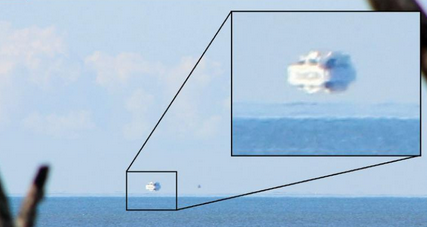
\includegraphics[scale=1]{Images/Cours/Chapitre_4/Mirage.PNG}
\end{center}
\begin{center}
     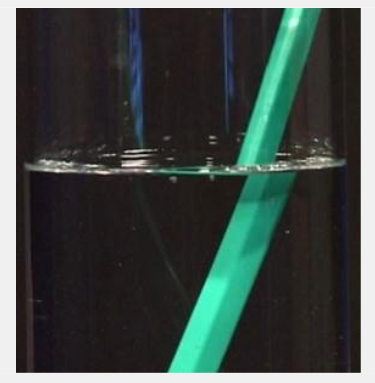
\includegraphics[scale=1]{Images/Cours/Chapitre_4/Crayon_brise.PNG}
\end{center}
Un crayon posé dans un verre d'eau semble se briser lors de son passage dans le verre ...
\end{multicols}
\textbf{Cela est dû au changement du milieu de propagation de la lumière !}
%    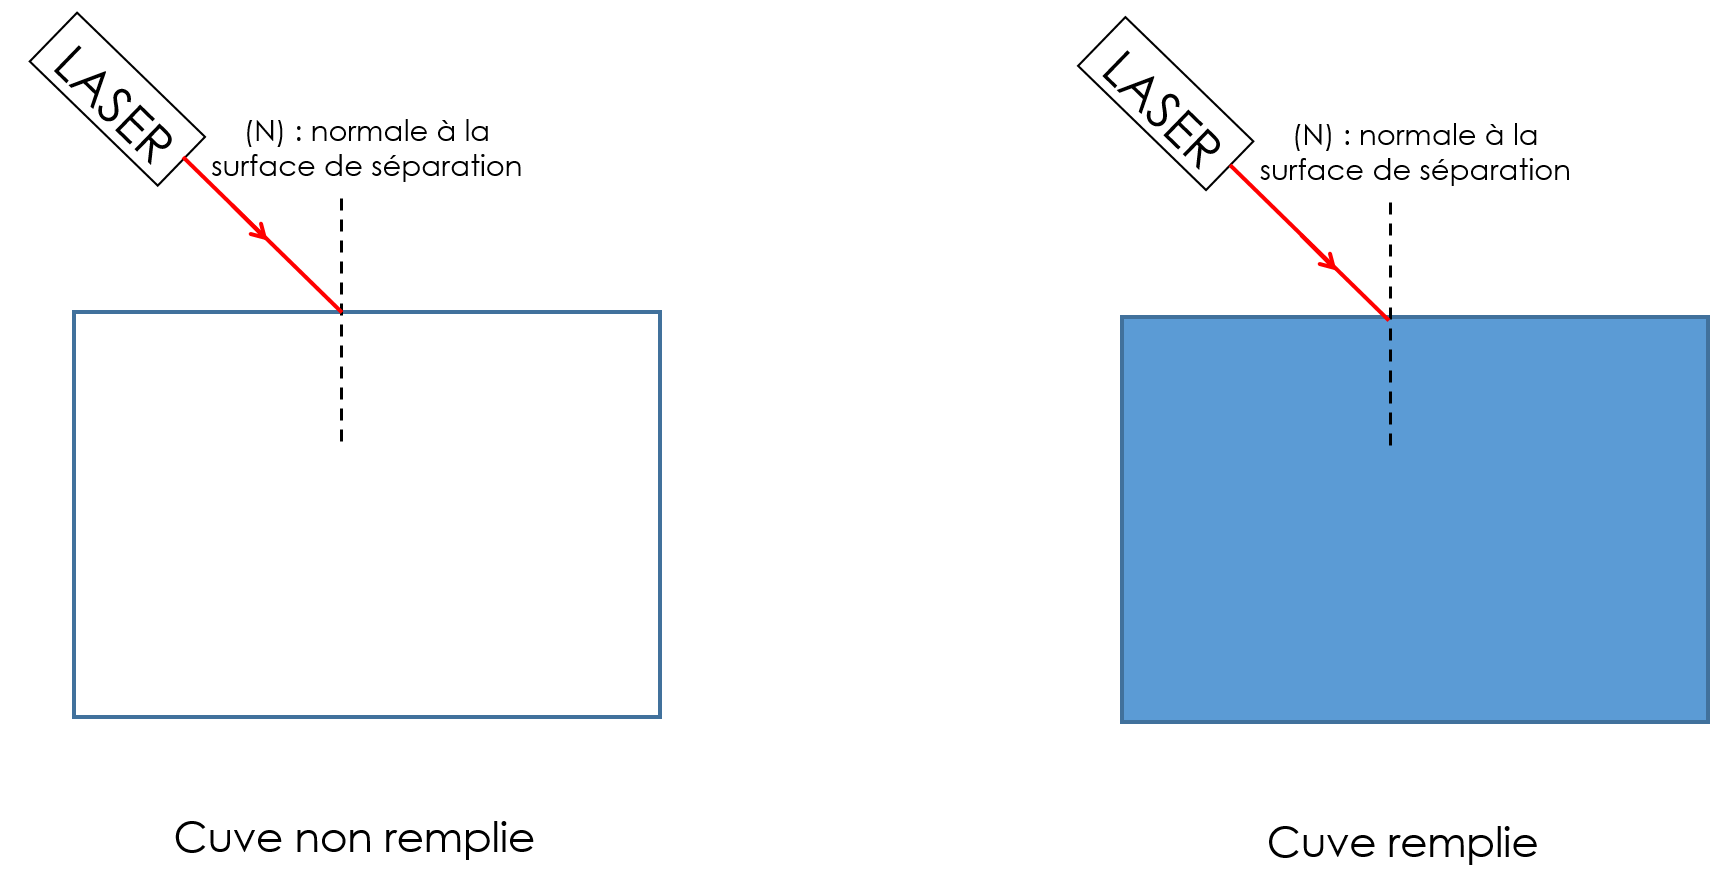
\includegraphics[scale=0.5]{Images/TP/TP9/Experience_intro.png}
%\end{center}
%\begin{wrapfigure}{r}{0.3\textwidth}
%\vspace{-0cm}
%    \centering
%     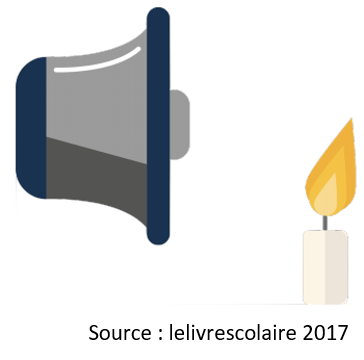
\includegraphics[width=0.32\textwidth]{Images/Cours/Chapitre_3/Haut_parleur_bougie.PNG}
%   \end{wrapfigure}
%\textcolor{green}{\underline{Expérience 1 :}} On place un laser face à une cuve vide. On vaporise de l'eau sur le trajet de la lumière. Observations : \\
%\textcolor{red}{En vaporisant de l'eau sur le parcours de la lumière, on observe que \underline{la lumière se propage en ligne droite}.}\\
%\textcolor{green}{\underline{Expérience 2 :}} Cette fois, on remplit la cuve d'un mélange eau-fluoréscine qui permet de visualiser le trajet de la lumière. Observations : \\
%\textbf{Observations :} \textcolor{red}{Par rapport à l'expérience 1, on remarque que la lumière du laser n'arrive pas au même endroit sur l'écran. Elle a été \underline{déviée}.}

\subsection{Représentation de la situation}
\begin{center}
    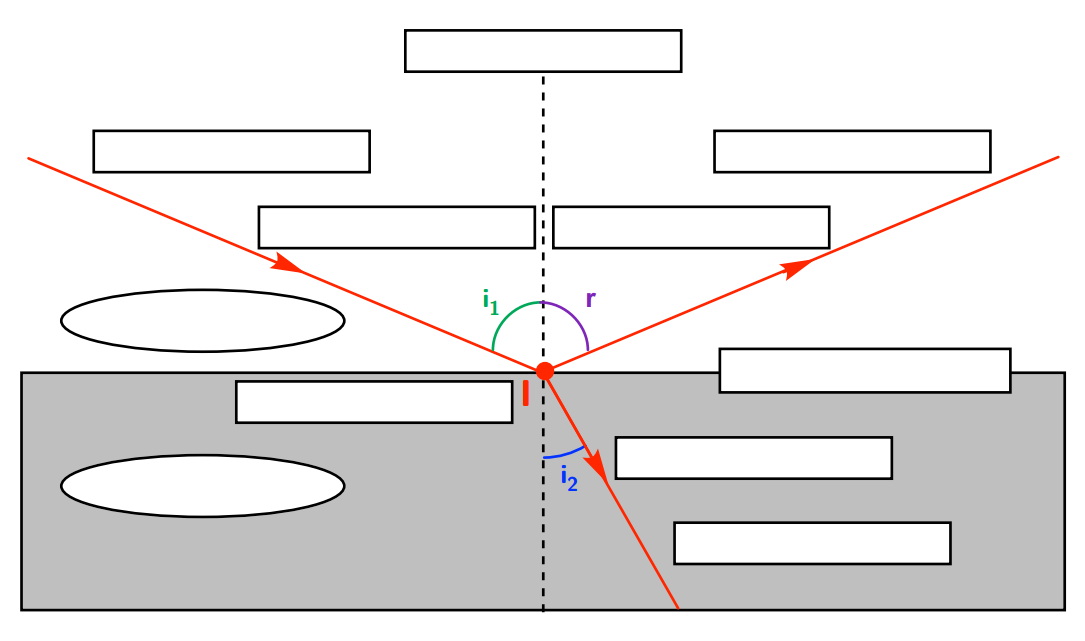
\includegraphics[scale=0.7]{Images/Cours/Chapitre_4/Schema_changement_milieu.PNG}
\end{center}

\subsection{Les lois de Snell-Descartes}
\subsubsection{Loi sur la réflexion}
\begin{tcolorbox}[colback=red!5!white,colframe=red!75!black,title=\textbf{1$^{\text{ère}}$ loi de Snell-Descartes :}, upperbox=invisible]
Le rayon incident et le rayon réfléchi appartiennent au même plan appelé \textcolor{red}{plan d'incidence}.\\
L'angle d'incidence $i_1$ et l'angle de réflexion $r$ sont égaux :
\begin{empheq}[box=\fbox]{equation*}
    i_1=r
\end{empheq}
\end{tcolorbox}

\subsubsection{Loi sur la réfraction}
Lors du passage du milieu d'incidence au milieu de réfraction, la lumière est déviée : c'est le phénomène de \textcolor{red}{réfraction}.
\begin{tcolorbox}[colback=red!5!white,colframe=red!75!black,title=\textbf{2$^{\text{ème}}$ loi de Snell-Descartes :}, upperbox=invisible]
Le rayon incident, réfracté appartiennent au même plan appelé \textcolor{red}{plan d'incidence}.\\
L'angle d'incidence $i_1$ et l'angle de réfraction $i_2$ sont reliés par la formule suivante :
\begin{empheq}[box=\fbox]{equation*}
    n_1 \sin\left(i_1\right)= n_2 \sin\left(i_2\right)
\end{empheq}
\end{tcolorbox}

\begin{center}
    \begin{tabular}{|c|C{0.15}|C{0.13}|C{0.15}|C{0.17}|C{0.15}|}
        \hline
        \cellcolor{blue!25}Milieu & vide & air & eau & plexiglas (TP 9) & diamant \\
        \hline
         \cellcolor{blue!25}Indice optique n & 1 (exactement) & 1,00 & 1,33 &  & 2,52 \\
         \hline
    \end{tabular}
\end{center}
\begin{Large}
    \ding{45}
\end{Large}\textbf{Exercice 9, 10, 11, 12, 22, 29, 31}

\subsection{Dispersion de la lumière}
\begin{Large}
    \ding{43}
\end{Large}
Voir \textit{TP 10 : L'apparition d'un arc-en-ciel}.
\begin{multicols}{2}
    \begin{center}
        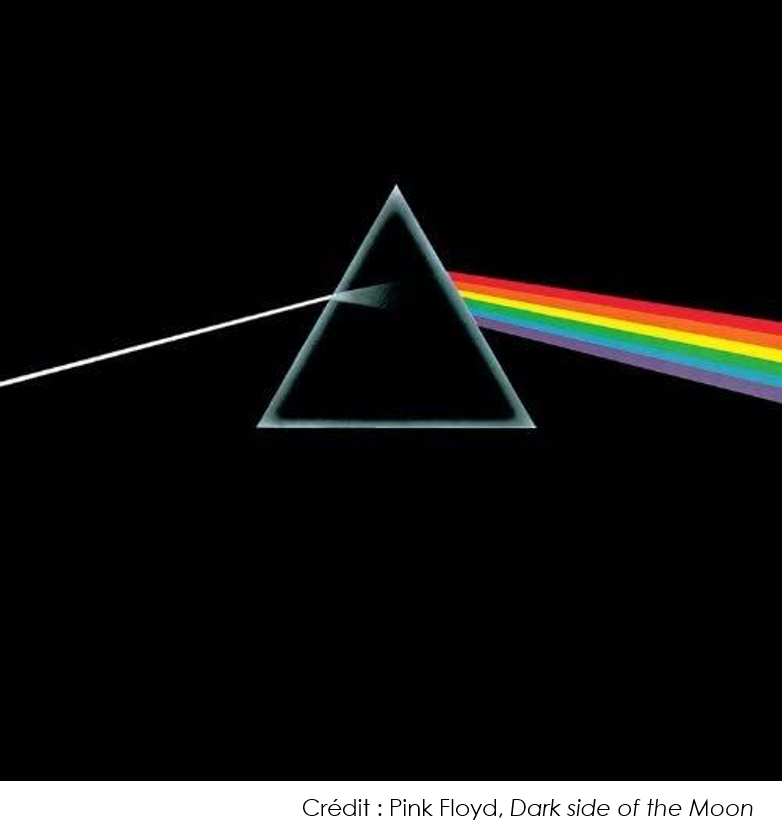
\includegraphics[scale=0.5]{Images/Cours/Chapitre_4/Pink_floyd.png}
    \end{center}
    
    \begin{tcolorbox}[colback=green!5!white,colframe=green!75!black,title=\textbf{Milieu dispersif et spectre:}, upperbox=invisible]
Un milieu est dit \textcolor{red}{disersif} si son indice optique $n$ dépend de la longueur d'onde (c'est-à-dire de la couleur) de la lumière qui le traverse.\\

L'image de cette décomposition des couleurs sur un écran est appelé le \textcolor{red}{spectre de la lumière blanche}.
\end{tcolorbox}
\end{multicols}

\begin{tcolorbox}[colback=green!5!white,colframe=green!75!black,title=\textbf{Source monochromatique ou polychromatique:}]
Une source de lumière est dite \textcolor{red}{monochromatique} si elle produit une lumière composée d'une seule longueur d'onde. Par exemple : un laser.\\

Une source de lumière est dite \textcolor{red}{polychromatique} si elle produit une lumière composée de plusieurs longueurs d'ondes. Par exemple : le soleil.
\end{tcolorbox}

\begin{Large}
    \ding{45}
\end{Large}\textbf{Exercice 14, 19}
\section{Modélisation de l'\oe il par une lentille}
\begin{Large}
    \ding{43}
\end{Large}
Voir \textit{Activité : L'\oe il, un instrument remarquable}.

\subsection{Modélisation}
Tout comme une lentille, l'\oe il permet de visualiser un \textcolor{red}{objet} à une certaine distance en faisant converger les rayons lumineux issus de cet objet pour en produire une \textcolor{red}{image} sur la rétine :
\begin{center}
    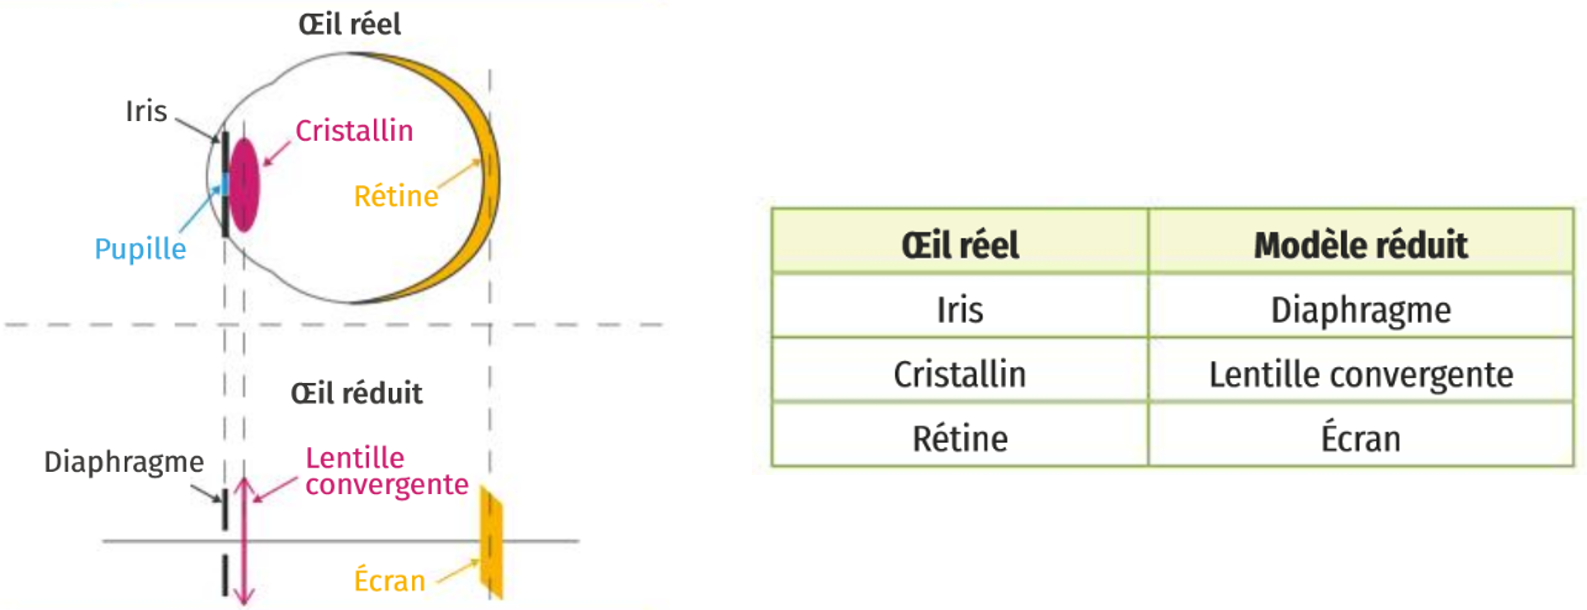
\includegraphics[scale=0.5]{Images/Cours/Chapitre_4/Modele_oeil.PNG}
\end{center}

\subsection{Détermination graphique d'une image par une lentille convergente}

\begin{tcolorbox}[colback=green!5!white,colframe=green!75!black,title=\textbf{Lentille convergente :}]
\begin{multicols}{2}
    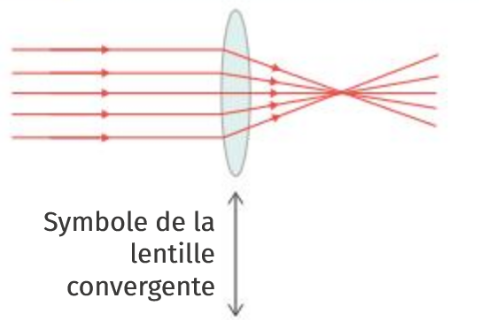
\includegraphics[scale=0.7]{Images/Cours/Chapitre_4/Lentille.PNG}
    
    %Une lentille est caractérisée par son \textcolor{red}{centre optique} O par lequel passe l'axe optique $\Delta$, son \textcolor{red}{foyer image} F' et \textcolor{red}{son foyer objet} F.
\end{multicols}
\end{tcolorbox}

\begin{tcolorbox}[colback=red!5!white,colframe=red!75!black,title=\textbf{Construction d'une image par une lentille :}]
\begin{itemize}
    \item Le rayon passant par le centre optique O \textbf{n'est pas dévié} ;
    \item Les rayons arrivant parallèlement à l'axe optique $\Delta$ \textbf{ressortent sur le foyer image F'} ;
    \item Les rayons passant par le foyer objet F \textbf{ressortent parallèle à l'axe optique $\Delta$}.
\end{itemize}
\end{tcolorbox}

\begin{center}
    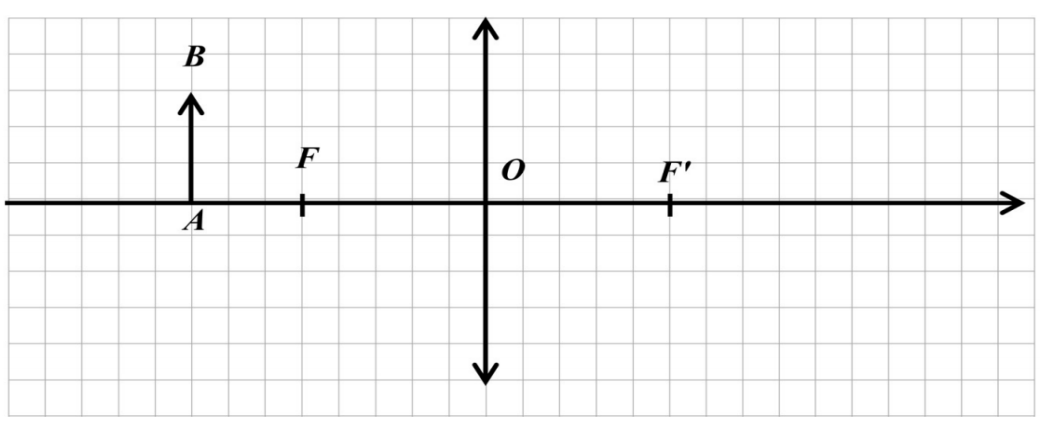
\includegraphics[scale=1]{Images/Cours/Chapitre_4/Lentille_construction_eleve.PNG}
\end{center}

\subsection{Grandissement}
Pour un objet de taille AB, on obtient une image A'B'. \begin{tcolorbox}[colback=green!5!white,colframe=green!75!black,title=\textbf{Grandissement :}, upperbox=invisible]
On définit le \textcolor{red}{grandissement} $\gamma$ d'une lentille comme le rapport entre la \textcolor{red}{hauteur algébrique} de l'image $\overline{\text{A'B'}}$ sur la \textcolor{red}{hauteur algébrique} de l'objet $\overline{\text{AB}}$ :
\begin{empheq}[box=\fbox]{equation*}
    \gamma = \frac{\overline{A'B'}}{\overline{AB}}
\end{empheq}
\begin{itemize}
    \item Si $\gamma$ est négatif, alors l'image est renversée ;
    \item Si $\abs{\gamma}$ est plus petit que 1, alors l'image est rétrécie.
\end{itemize}
\end{tcolorbox}

\begin{mdframed}[style=autreexo]
\textbf{\bsc{Exercice de cours} - Grandissement}\\
Sur la construction précédente, déterminer $\gamma$.
\end{mdframed}

\begin{Large}
    \ding{45}
\end{Large}\textbf{Exercice 25, Appareil photo}